%tag:000U
%label:"art:lagrangianSurgery"
%author:JeffHicks
%name:"surgery of Lagrangian submanifolds "
%type:"article"

We will now look at some ways to glue together new Lagrangian submanifolds from old.
A source of inspiration for us will be from smooth topology, where tools such as surgery, Morse theory, and cobordisms provide methods for generating new manifolds.
An example where we can take a method from topology and directly import it into symplectic geometry is connect sum for Lagrangian curves inside of surfaces.
In this setting, two Lagrangian curves which intersect at a point are modified at the point of intersection to produce a connected Lagrangian submanifold.
See \cref{fig:connectsumcurve}.

The Polterovich connect sum is a generalization of this surgery to higher dimensions, which smooths out a transverse intersection between two Lagrangian submanifolds. 
The idea of construction is to first use \cref{lemma:straightening} to provide a canonical neighborhood for a transverse Lagrangian intersection, then construct a model neck in that canonical neighborhood. 
%tag:000X
%label:"fig:polterovichSurgery"
%author:JeffHicks
%name:"Polterovich Surgery"
%type:"figure"
%parent:prp:polterovichSurgery
%caption:"The connect sum of two Lagrangian curves in a surface"

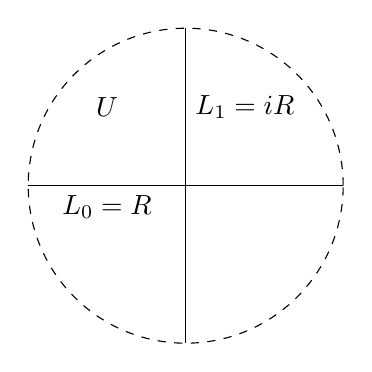
\begin{tikzpicture}
      \draw[dashed]  (0,0) circle[radius=2];
      \draw (-2,0) -- (2,0) (0,2) -- (0,-2);
      \node at (-1,1) {$U$};
      \node[right] at (0,1) {$L_1=i\mathbb R$};
      \node[below] at (-1,0) {$L_0=\mathbb R$};
      \end{tikzpicture}
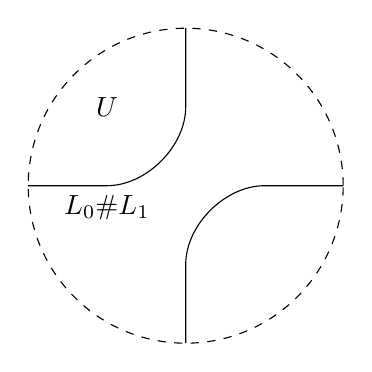
\begin{tikzpicture}
      \draw[dashed]  (0,0) circle[radius=2];
      \node at (-1,1) {$U$};
      
      \node[below] at (-1,0) {$L_0\#L_1$};
      
      \draw (-2,0) .. controls (-1.5,0) and (-1.5,0) .. (-1,0) .. controls (-0.5,0) and (0,0.5) .. (0,1) .. controls (0,1.5) and (0,1.5) .. (0,2) ;
      \draw (2,0) .. controls (1.5,0) and (1.5,0) .. (1,0) .. controls (0.5,0) and (0,-0.5) .. (0,-1) .. controls (0,-1.5) and (0,-1.5) .. (0,-2);
      
\end{tikzpicture}

%tag:000T
%label:"prp:polterovichSurgery"
%author:JeffHicks
%name:"Polterovich surgery of Lagrangian submanifolds"
%type:"proposition"
%source:"polterovich1991surgery"

Let $L_1, L_2\subset X$ be two Lagrangian submanifolds intersecting transversely at a single point $p$. 
Then there exists a Lagrangian submanifold $L_1\#_p L_2\subset X$ which
\begin{itemize}
        \item topologically is the connect sum of $L_1$ and $L_2$ at $p$. 
        \item Agrees with $L_1\cup L_2$ outside of a small neighborhood of $p$ in the sense that 
        \[L_1\#_p L_2|_{X\setminus U}=L_2\cup L_2|_{X\setminus U}.\]
\end{itemize}
 
%tag:000L
%label:"prf:polterovichSurgery"
%author:JeffHicks
%name:"construction of Polterovich surgery"
%type:"proof"
%parent:prp:polterovichSurgery

 
 

By \cref{lemma:straightening}, it suffices to construct the Lagrangian surgery neck replacing the a standard intersection neighborhood $X=\CC^n$, $L_1=\RR^n$ and $L_2=\jmath\RR^n$.
We start by picking a \emph{surgery profile curve},  
\begin{align*}
      \gamma: [-R, R] \to& \CC\\
      t\mapsto& (a(t)+\jmath b(t))
\end{align*}
with the property that $a(t), b(t)$ are non-decreasing, $\gamma(t)=t$ for $t$ sufficiently small, and $\gamma_\lambda(t)=\jmath t$ for $t$ sufficiently large. We ask that the area between the real axis, imaginary axis, and $\gamma$ is $\lambda$.
An example is drawn in \cref{fig:polterovichSurgeryProfile}.
%label:"fig:polterovichSurgeryProfile"
%author:JeffHicks
%name:"surgery profile"
%type:"figure"
%parent:"def:polterovichSurgery"
%caption:"Surgery Profile for Polterovich surgery"



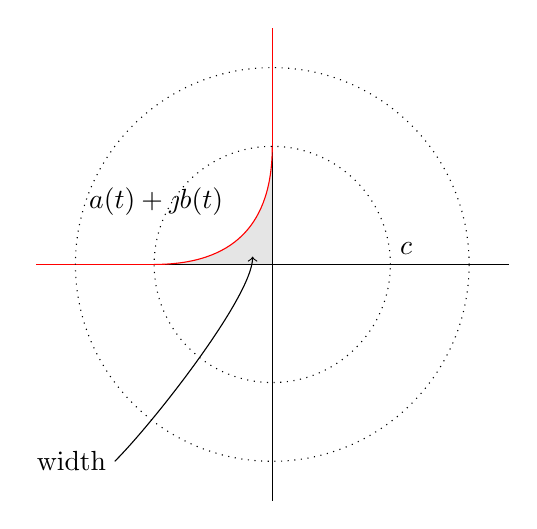
\begin{tikzpicture}

    \fill[fill=gray!20] (-1.5,0) .. controls (-0.5,0) and (-0.5,0) .. (0,0) .. controls (0,0.5) and (0,0.5) .. (0,1.5) .. controls (0,0.5) and (-0.5,0) .. (-1.5,0);
    
    \draw (0,3) -- (0,-3);
    \draw (3,0) -- (-3, 0);
    \draw[red] (-3, 0)--(-1.5,0) (0,1.5)--(0, 3);
    \draw[red] (-1.5,0) .. controls (-0.5,0) and (0,0.5) .. (0,1.5);
    \node[above left] at (-0.5,0.5) {$a(t)+\jmath b(t)$};
    \node[above right] at (1.5,0) {$c$};
    \draw[dotted]  (0,0) ellipse (1.5 and 1.5);
    \draw[dotted]  (0,0) ellipse (2.5 and 2.5);
    \draw[->] (-2,-2.5) .. controls (-1.5,-2) and (-0.25,-0.4) .. (-0.25,0.1);
    \node at (-2.55,-2.5) {width};
\end{tikzpicture}
This neck provides a local model for the Lagrangian surgery, which is the Lagrangian surgery neck:
\[
	L_1\#_\gamma L_2:=\left\{(\gamma(t)\cdot x_1,\ldots,  \gamma(t)\cdot x_n \text{ such that } x_i \in \RR^n,t\in \RR, \sum_{i} x_i^2=1\right\}.
\]
Note that when $t$ is sufficiently small this parameterizes $(\RR\setminus B_r(0))\subset \CC^n$, and when $t$ is sufficiently large this parameterizes $(\jmath \RR \setminus B_r(0))\subset \CC^n$. 
Therefore, this construction satisfies the condition that the surgery Lagrangian agrees with the surgery components outside of a small neighborhood of the surgery point.
This Lagrangian has the topology of $S^{n-1}\times \RR$, which is the local model for the connect sum $\RR^n\#_0\RR^n$.

It remains to show that the submanifold is Lagrangian \todo{}


The Lagrangian is then taken to be $L_1\#_\gamma L_2$ for any suitable choice of $\gamma$.
 
One feature of surgery is that it does not uniquely specify a Lagrangian --- different choices of curves $\gamma$ produce different Lagrangian submanifolds.
Recall that to a Lagrangian isotopy $\li_t: L\to C$ we associate a cohomology class $\Flux_{\li_t}\in H^1(L)$. 
We can similarly associate a flux class to a Lagrangian surgery.
A given surgery profile curve $\gamma$ can be extended to a family of Lagrangian surgery profiles by scaling the profile curve by a parameter $s$.  
This gives us a family of surgeries $L_1\#_{s\gamma} L_2$, which are Lagrangian isotopic.
The flux of the surgery is defined to be the flux of this isotopy. 
%label:"prp:fluxOfSurgery"
%author:JeffHicks
%name:"flux of Polterovich surgery"
%type:"proposition"

Let $L_0, L_1$ be two Lagrangian submanifolds which intersect transversely at a point, and let $U$ be a neighborhood of the point in which we implant a surgery neck. Suppose two profile curves $\gamma_0, \gamma_1$ have the same flux $\lambda$.
Then there exists a Hamiltonian supported on $U$ whose time one identifies $L_1\#_{\gamma_0} L_2$ and $L_1\#_{\gamma_1} L_2$.
As a result, we will write $L_1\#_{\lambda}L_2$ for a curve where the profile curve $\gamma$, real axis and imaginary axis bound a region of area $\lambda$. 

The order of the summands plays an important role in Lagrangian surgery, as it is generally the case that $L_1\#L_2$ and $L_2\#L_1$ are not Lagrangian isotopic. 
%label:"exm:polterovichSurgery"
%author:JeffHicks
%name:"Polterovich surgery in $\RR^n$"
%type:"example"


We now visualize the Polterovich surgery for Lagrangian sections of $T^*\RR^n$.
The Lagrangians which we consider are two sections of the cotangent bundle. 
Let $L_1$ be the graph of $d(q_1^2+ \cdots+ q_n^2)$, and let $L_2$ be the graph of $d(-q_1^2-\cdots -q_n^2)$. 
In dimension 2, we can then draw $L_1\# L_2$ and $L_2\# L_1$ as multisections of the cotangent bundle. 
These multisections are sketched in \cref{fig:surgeryDim4}.
Note that one of surgeries creates a Lagrangian which has a ``neck'' visible in the projection to the base of the cotangent bundle.
The other surgery is generically a double-section of the cotangent bundle, except over the fiber of the intersection point where it is instead an $S^1$.


%label:"fig:surgeryDim4"
%author:JeffHicks
%name:"surgery of Lagrangians in $\dim(X)=2"
%type:"figure"
%parent:"con:dehnTwist"
%caption:"Lagrangian surgery of two sections of $T^*\RR^2$"


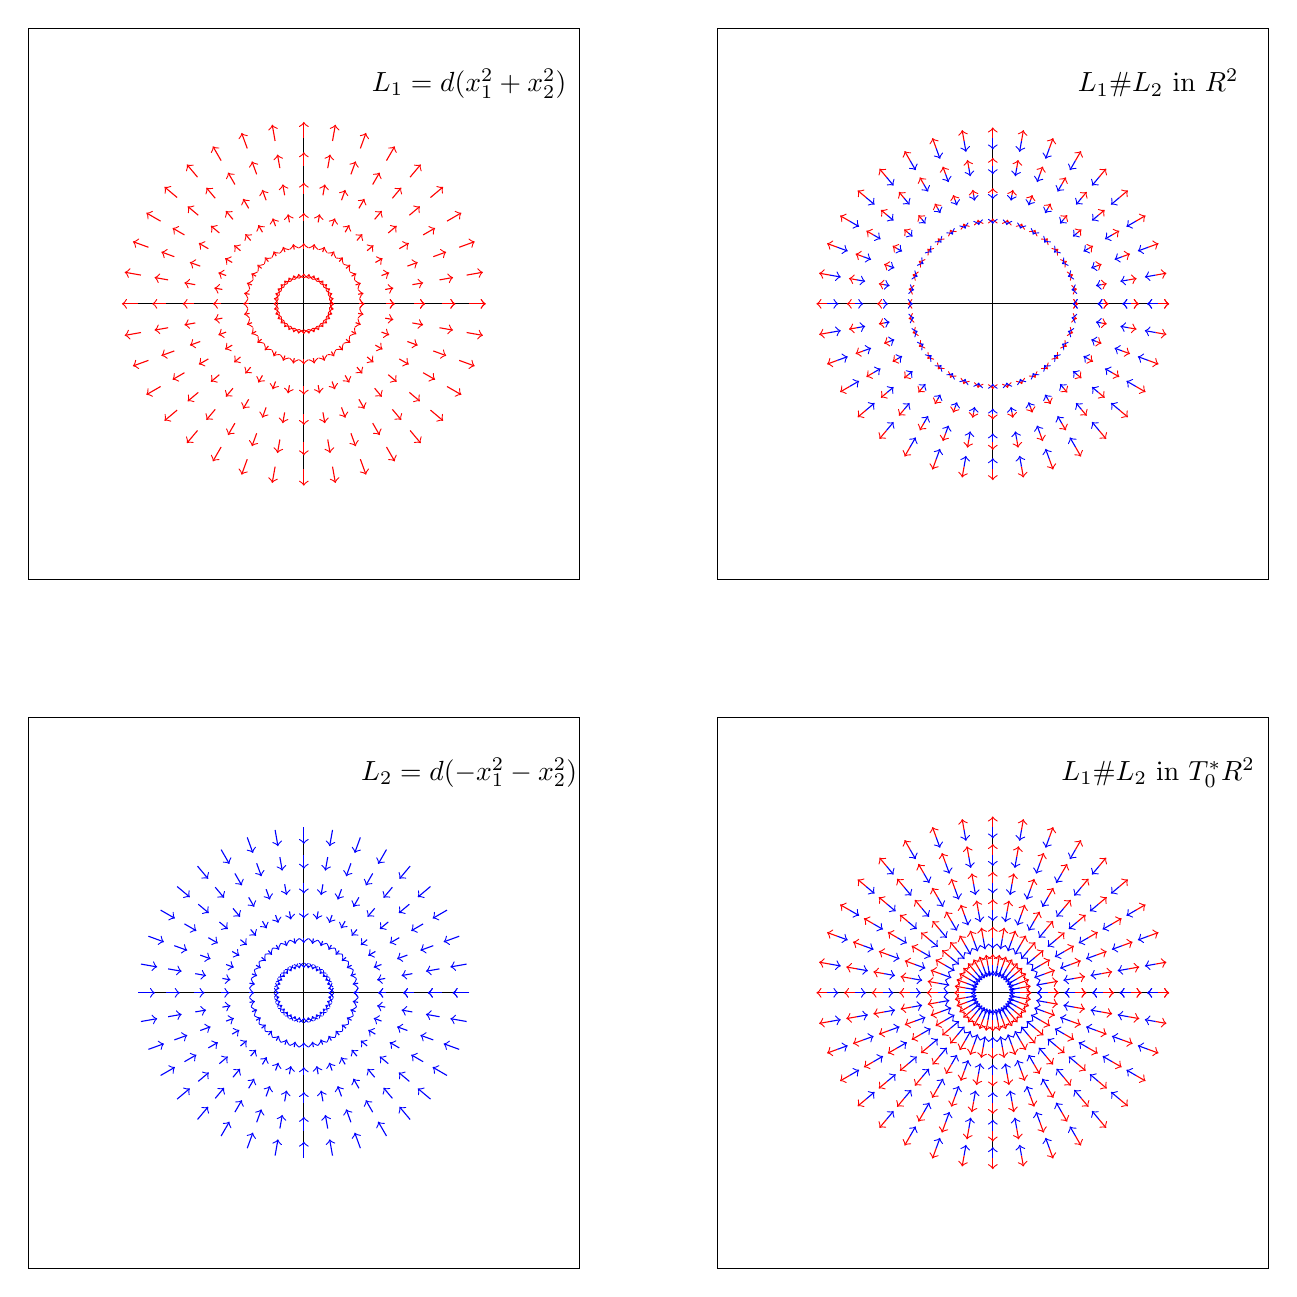
\begin{tikzpicture}[scale=.7]


    \begin{scope}[shift={(-12.5,1)}]
    \draw  (-5,5) rectangle (5,-5);
    \node at (3,4) {$L_1= d(x^2_1+x_2^2)$};
    
    \begin{scope}
    \draw (-3,0)--(3,0) (0,3)--(0,-3);
    \foreach \r in { .5, 1,1.5, 2,2.5, 3} {
        \foreach \t in {0,...,36} {
            \draw[->, red] ({\r * cos(10*\t)},{ \r * sin(10*\t) })-- ({1.1*\r * cos(10*\t)},{ 1.1*\r * sin(10*\t) });
            %\draw[->, blue] ({\r * cos(10*\t)},{ \r * sin(10*\t) })-- ({0.9*\r * cos(10*\t)},{ 0.9*\r * sin(10*\t) });
        }
    }
    \end{scope}
    \end{scope}
    
    
    \begin{scope}[shift={(-12.5,-11.5)}]
    
    
    \draw  (-5,5) rectangle (5,-5);
    
    \node at (3,4) {$L_2=d(-x^2_1-x_2^2)$};
        \begin{scope}
    \draw (-3,0)--(3,0) (0,3)--(0,-3);
    \foreach \r in { .5, 1,1.5, 2,2.5, 3} {
        \foreach \t in {0,...,36} {
            %\draw[->, red] ({\r * cos(10*\t)},{ \r * sin(10*\t) })-- ({1.1*\r * cos(10*\t)},{ 1.1*\r * sin(10*\t) });
            \draw[->, blue] ({\r * cos(10*\t)},{ \r * sin(10*\t) })-- ({0.9*\r * cos(10*\t)},{ 0.9*\r * sin(10*\t) });
        }
    }
    \end{scope}
    \end{scope}
    
    \begin{scope}[]
    
    \begin{scope}[shift={(0,1)}]
    
    
    \draw  (-5,5) rectangle (5,-5);
    
    \node at (3,4) {$L_1\#L_2$ in $\mathbb R^2$};
    
    
    
    \begin{scope}
    \draw (-3,0)--(3,0) (0,3)--(0,-3);
    \foreach \r in { .5, 1,1.5, 2} {
        \foreach \t in {0,...,36} {
            \draw[->, red] ({(\r+1) * cos(10*\t)},{ (\r+1) * sin(10*\t) })-- ({(1.1*\r +1)* cos(10*\t)},{ (1.1*\r+1) * sin(10*\t) });
            \draw[->, blue] ({(\r+1) * cos(10*\t)},{ (\r+1) * sin(10*\t) })-- ({(0.9*\r+1) * cos(10*\t)},{( 0.9*\r +1)* sin(10*\t) });
        }
    }
    \end{scope}
    \end{scope}
    \begin{scope}[shift={(0,-11.5)}]
    
    
    \draw  (-5,5) rectangle (5,-5);
    
    \node at (3,4) {$L_1\#L_2$ in $T^*_0\mathbb R^2$};
    
    \begin{scope}
    \draw (-3,0)--(3,0) (0,3)--(0,-3);
    \foreach \r in {.5, 1,1.5, 2,2.5, 3} {
        \foreach \t in {0,...,36} {
            \draw[->, red] ({\r * cos(10*\t)},{ \r * sin(10*\t) })-- ({(\r+.2) * cos(10*\t)},{ (\r+.2) * sin(10*\t) });
            \draw[->, blue] ({\r * cos(10*\t)},{ \r * sin(10*\t) })-- ({(\r-.2) * cos(10*\t)},{ (\r-.2) * sin(10*\t) });
        }
    }
    \end{scope}
    \end{scope}
    
    \end{scope}
    
    \end{tikzpicture}


 



Now that we have a geometric description of $L_1\#_\lambda L_2$, we discuss what object it represents in the Fukaya category. We restrict ourselves to $\dim_\CC(X)=1$ so that we may draw pictures (but the construction works in higher dimensions as well).

Let $L_0$ be some test Lagrangian, which intersects both $L_1$ and $L_2$ as in \cref{fig:roundingCorner}. If the surgery neck is chosen to lie in a neighborhood disjoint from the intersections  $L_0\cap (L_1\cup L_2)$, then these intersections are in bijection with the intersections $L_0\cap (L_1\# L_2)$.
%label:"fig:roundingCorner"
%author:JeffHicks
%name:"rounding corner in Polterovich surgery"
%type:"figure"
%parent:"thm_roundingCorner"
%caption:"By rounding the corner, we can compare holomorphic triangles with holomorphic strips on the surgery."


    
    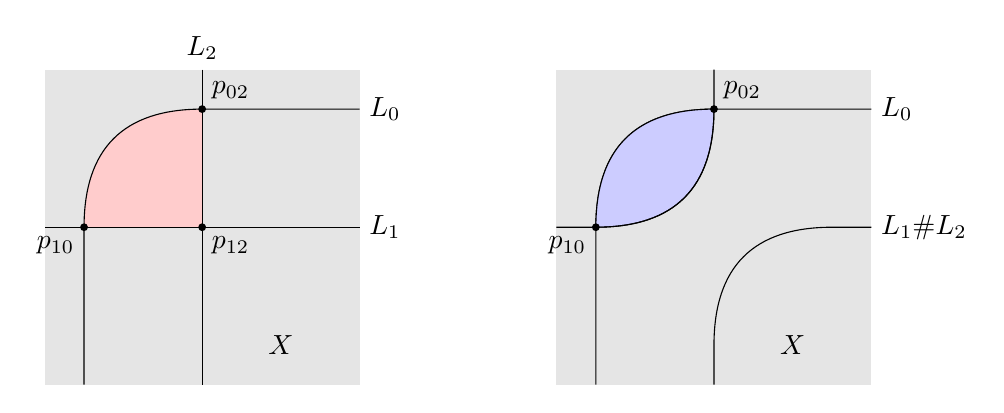
\begin{tikzpicture}\begin{scope}[]
    
    
        \fill[gray!20]  (-2,2) rectangle (2,-2);
        \fill[red!20] (0,0) .. controls (0,0.5) and (0,1) .. (0,1.5) .. controls (-1,1.5) and (-1.5,1) .. (-1.5,0) .. controls (1,0) and (0.5,0) .. (0,0);
        
        \draw (0, 2)--(0,-2);
        \draw (2,0) -- (-2,0);
        \draw (2,1.5) .. controls (1,1.5) and (0.5,1.5) .. (0,1.5) .. controls (-1,1.5) and (-1.5,1) .. (-1.5,0) .. controls (-1.5,-0.5) and (-1.5,-1.5) .. (-1.5,-2);
        
        \node[right] at (2,1.5) {$L_0$};
        \node[right] at (2,0) {$L_1$};
        \node[above] at (0,2) {$L_2$};
        \node[below right] at (0,0) {$p_{12}$};
    \node[above right] at (0,1.5) {$p_{02}$};
    \node[below left] at (-1.5,0) {$p_{10}$};
        \node[fill=black, circle, scale=.3] at (0,0) {};
        \node[fill=black, circle, scale=.3] at (0,1.5) {};
        \node[fill=black, circle, scale=.3] at (-1.5,0) {};
    \node at (1,-1.5) {$X$};
    \end{scope}
        
        
        \begin{scope}[shift={(6.5,0)}]
        
        
        \fill[gray!20]  (-2,2) rectangle (2,-2);
        \draw (2,1.5) .. controls (1,1.5) and (0.5,1.5) .. (0,1.5) .. controls (-1,1.5) and (-1.5,1) .. (-1.5,0) .. controls (-1.5,-0.5) and (-1.5,-1.5) .. (-1.5,-2);
        
        \node[right] at (2,1.5) {$L_0$};
        \node[right] at (2,0) {$L_1\#L_2$};
        
        
        \draw[fill=blue!20] (0,1.5) .. controls (0,0.5) and (-0.5,0) .. (-1.5,0) .. controls (-1.5,1) and (-1,1.5) .. (0,1.5);
        
        \draw (0,2) .. controls (0,1.5) and (0,2) .. (0,1.5) .. controls (0,0.5) and (-0.5,0) .. (-1.5,0) .. controls (-2,0) and (-2,0) .. (-2,0);
        \draw (0,-2) .. controls (0,-2) and (0,-2) .. (0,-1.5) .. controls (0,-0.5) and (0.5,0) .. (1.5,0) .. controls (2,0) and (2,0) .. (2,0);
        
        
    \node[above right] at (0,1.5) {$p_{02}$};
    \node[below left] at (-1.5,0) {$p_{10}$};
        \node[fill=black, circle, scale=.3] at (0,1.5) {};
        \node[fill=black, circle, scale=.3] at (-1.5,0) {};
    \node at (1,-1.5) {$X$};
        \end{scope}
        
        \end{tikzpicture}
 The intuition from \cite{fukaya2007lagrangian} is that there is a bijection between certain holomorphic triangle with boundary on $L_0, L_1, L_2$ which passes through the intersection point $p_{12}$, and holomorphic strips with boundary on $L_0$ and $L_1\# L_2$. Since holomorphic triangles contribute to the $\emprod^3$ structure coefficients, and strips to the differential, it is reasonable to hope that we can state a relation between $L_1, L_2,$ and $L_1\#L_2$ as objects of the Fukaya category.


First, we observe that the intersection point $p_{12}$ determines a morphism in $\hom(L_2, L_1)$. Since we've assumed that $L_1$ and $L_2$ intersect at only one point, we know that $\emprod^1(p_{12})=0$. We can therefore form the twisted complex $\cone(p_{12})$. We now provide justification for why this is isomorphic to $L_1\# L_2$.

We have already observed that for our test Lagrangian $L_0$ we had an isomorphism of vector spaces between $\hom(L_0, L_1)\oplus \hom(L_0, L_2)$ and $\hom(L_0, L_1\#_{p_{12}}L_2)$. The differential on $\hom(L_0, L_1\#_{p_{12}}L_2)$ comes counting holomorphic strips, which we break into two types: those which avoid a neighborhood of the surgery neck, and those which pass through the surgery neck. 
%label:prp:stripsInLagrangianSurgery
%name:"strips with boundary on Lagrangian surgery avoiding the neck"
%type:proposition


If $\dim_\RR(X)\geq 4$, then we can choose an almost complex structure $J$ so that whenever $p_{01}, q_{01}\in L_0\cap L_1$ are intersections, and $u: [0,1]\times \RR\to X$ is a $J$ holomorphic strip, then the boundary of $u$ is disjoint from a small neighborhood of $L_1\cap L_2$. In particular, $u$ gives a $J$-holomorphic strip with boundary on $L_0, L_1\#_{p_{12}} L_2$.

The more difficult portion is to understand the strips which pass through the neck.
%label:"thm:roundingCorner"
%author:JeffHicks
%name:"rounding the corner"
%type:"theorem"
%source:"fukaya2007lagrangian"


    Let $\dim(X)\geq 4$, and $L_1, L_2$ be exact Lagrangian submanifolds which intersect transversely at a single point $p_{12}$. Let $L_0$ be another exact Lagrangian submanifold which intersects $L_1, L_2$ transversely. Then for sufficiently small surgery necks, there exists a choices of almost complex structure on $X$ for which we have a bijection between
    \begin{itemize}
        \item $J$-holomorphic strips with boundary on $L_0, L_1\# L_2$ which pass through the surgery neck;
        \item $J$-holomorphic triangles with boundary on $L_0, L_1, L_2$.
    \end{itemize}

From this we obtain the following corollary
%label:cor:surgeryExactTriangle
%author:JeffHicks
%name:"surgery exact Triangle"
%type:corollary
%

\begin{corollary}
    Let $\dim(X)\geq 4$, and $L_1, L_2$ be Lagrangians which intersect transversely at a single point $p_{12}$. Then $L_1\#_{\lambda} L_2$ is isomorphic to the twisted complex $(L_1[1]\oplus L_2, \emprod^2(p_{12}-)).$
\end{corollary}
